
%=======================================================================
% Theoretische perfromantie hoofdstuk
%=======================================================================

\chapter{\IfLanguageName{dutch}{Theoretische performantie}{Theoretic performance}}
\label{ch:theoretischePerformantie}

\section{\IfLanguageName{dutch}{Metingen zijn belangrijk}{Measurements are important}}
\label{sec:importantMetrics}

Metingen zijn de basis waarop optimalisaties worden uitgevoerd, dit is in het geval van performantie niet anders. Weten waar werkpunten liggen en op basis daarvan een plan van aanpak opstellen zorgt voor doelgerichte optimalisatie. Arbitrair verandering aanbrengen zonder een duidelijke kijk te hebben op wat noodzakelijk is stelt zichzelf in vraag.

\subsection{\IfLanguageName{dutch}{De grootste factor}{The biggest factor}}
\label{sec:biggestFactor}

In de sectie~\ref{sec:whyPerformance} op pagina~\pageref{sec:whyPerformance} werd er al nadruk gelegd op de impact die een slechte performantie kan achterlaten voor een bedrijf, maar wat de gebruiker vindt geeft het uiteindelijke verdict. Waar het om draait voor de hedendaagse gebruiker van het \gls{www} is snelheid. Gebruikers willen zoveel mogelijk informatie op hun beeld krijgen op een snelle en efficiënte manier. \\
In het artikel van~\textcite{Everts2016} werden conclusies getrokken uit Google Analytics en data van derde partijen die vrijwillig bereid waren hun specifieke data te delen. De conclusies waren unaniem, te lange laadtijd zorgt voor ontevredenheid bij de gebruiker. Trage sites (19 seconden laadtijd) hebben zeer korte gebruikerssessies en vervolgens ook een hoger debouncepercentage, waarbij snelle sites (5 seconden laadtijd) 70 procent langere gebruikerssessies en 35 procent minder debouncepercentage ondervinden.

\subsection{\IfLanguageName{dutch}{Metrieken}{Metrics}}
\label{sec:metrics}

Wat zij de metrieken waarmee rekening gehouden worden in welzijn van de gebruiker? Dit kan gaan van hoe snel de eerste pixels op het scherm verschijnen tot de reactietijd van een interactie die de gebruiker uitvoert.

\subsubsection{\IfLanguageName{dutch}{FCP (First Contentful Paint)}{FCP (First Contentful Paint)}}
\label{sec:fcp}

De tijd totdat een gebruiker iets visueel op het scherm te zien krijgt wordt is the frist contentful paint. Het is een maatstaf om een idee te geven wanneer de gebruiker voor het eerst inhoud zal te zien krijgen die hij of zij kan consumeren. 

\subsubsection{\IfLanguageName{dutch}{FMP (First Meaningful Paint)}{FCP (First Meaningful Paint)}}
\label{sec:fmp}

In aanvulling op een first contentful paint wordt ook rekening gehouden met de tijd tot het eerste deel van de website waar een gebruiker iets aan heeft, deze belangrijke delen van een website worden hero elementen genoemd. In tegenstelling tot first contentful, wat nog maar een enkel woord kan zijn dat op het scherm verschijnt, is the first meaningful veel verfijnder. Wanneer een gebruiker het belangrijkste deel van een website eerst te zien krijgt aan een verwachte snelheid zal er minder aandacht geschonken worden wanneer de rest van diezelfde pagina verschijnt. Waardoor een website veel sneller oogt.

\subsubsection{\IfLanguageName{dutch}{Interactie}{Interaction}}
\label{sec:interaction}

Interactie is een algemeen begrip en wordt onderverdeeld in verschillende criteria. Met het steeds sneller evolueren van de niche, dat het internet is, worden doelstelling opgelegd die de industrie verwacht behaald te zien. \\ 
In figuur~\ref{fig:InteractionSpeedTarget} op pagina~\pageref{fig:InteractionSpeedTarget} worden de doelstellingen in verband met interactie aangekaart, bron van deze informatie komt is het artikel van~\textcite{Taub2017}.

\begin{itemize}[label={}]
    \item \textbf{Time to interact}:
    Geeft een indicatie weer van de tijd die nodig is vooraleer de gebruiker interactie kan voeren met delen van de website, zoals bv. een input veld selecteren, doorklikken op een link, animaties starten,\dots \newline
    \item \textbf{Interaction frame rate}:
    Meeste schermen hebben een refresh snelheid van 60\gls{fps}, wanneer er onder 60 wordt gegaan kan dit snel aanzien worden als \textit{laggy} voor een gebruiker. De oorzaak hiervoor is vaak teveel schrijven/lezen of een verrommeling van het \gls{dom}. \newline
    \item \textbf{Interaction response time}:
    Een abstracte maatstaf voor de snelheid waarmee een interactie word waargenomen door de gebruiker. Hoe lager deze waarde ligt, hoe sneller een website zal waargenomen worden.
\end{itemize}

\begin{figure}[H]
    \tikz\node [drop shadow={
        shadow scale=0.98,
        shadow xshift=0ex,
        shadow yshift=0ex,
        opacity=0.1,
    }]
    {\fcolorbox{black}{white}{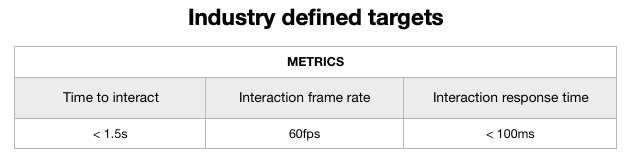
\includegraphics[width=\linewidth]{InteractionSpeedTarget}}};
    \caption{Verwachte waarden opgelegd door de industrie}
    \label{fig:InteractionSpeedTarget}
\end{figure}

\subsubsection{\IfLanguageName{dutch}{Laadproces}{Loading process}}
\label{sec:loadingProcess}

Wanneer een website wordt geladen worden er een bepaald aantal fasen doorlopen vooraleer de eerste pagina op het scherm tevoorschijn kan komen. In figuur~\ref{fig:browserPageLoadTimeline} op pagina~\pageref{fig:browserPageLoadTimeline} worden de fasen aangetoond op een as doorheen de tijd. Voor deze scriptie ligt de focus op frontend tijd.

\begin{itemize}[label={}]
    \item \textbf{\gls{dom} processing}:
    Na het verkrijgen van de \gls{html}, die via requests van de server werd gehaald, wordt deze omgezet naar een \gls{dom}. \newline
    \item \textbf{Pagina rendering}:
    Wanneer het \gls{dom} is aangemaakt begint de browser met het renderen van de pagina op basis van het \gls{dom}. In deze fase wordt de inhoud verwerkt en nadien kan de browser het window load event initialiseren.
\end{itemize}

\begin{figure}[h!]
    \tikz\node [drop shadow={
        shadow scale=0.98,
        shadow xshift=0ex,
        shadow yshift=0ex,
        opacity=0.2,
    }]
    {\fcolorbox{black}{white}{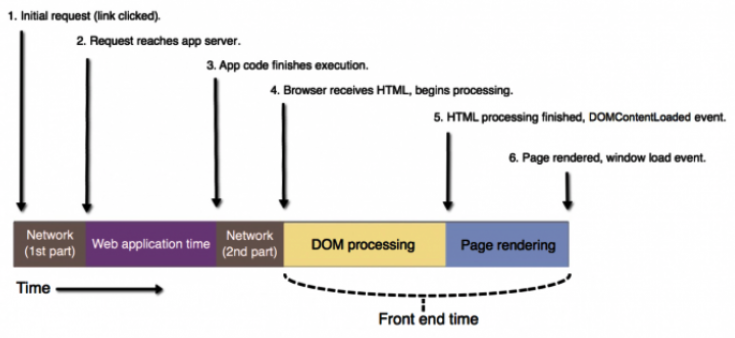
\includegraphics[width=\linewidth]{BrowserPageLoadTimeline.png}}};
    \caption{Tijdlijn voor het laden van een pagina, Bron:~\textcite{Relic2016}}
    \label{fig:browserPageLoadTimeline}
\end{figure}

\subsection{\IfLanguageName{dutch}{Tools}{Tools}}
\label{sec:testTools}

Zoals voordien al aangegeven in sectie~\ref{sec:biggestFactor} op pagina~\pageref{sec:biggestFactor} is snelheid alles bepalend en dit is te meten op basis van verschillende metrieken, welke al reeds besproken werden in sectie~\ref{sec:metrics} op pagina~\pageref{sec:metrics}. Voor het daadwerkelijk meten van deze maatstaven zijn er verschillende tools op de markt. Zo zijn er tools voor performantie tests manueel of geautomatiseerd kunnen zijn. Ook de Chrome DevTools bieden een geïntegreerde tool voor het testen van performantie. Hieronder enkele bekende voorbeelden van dergelijke tools: \\

\begin{itemize}[label={}]
    \item \textbf{MachMetrics}:
    Een tool die geautomatiseerde testresultaten voor snelheid dagelijks opmaakt en doorstuurt. Het is een best practice om de statistieken van je website op gepaste tijdstippen te analyseren. Het internet en daarbij ook websites zijn in continue verandering. \newline
    \item \textbf{WebPageTest}:
    Online platform voor het testen van allround performantie in verschillende browsers op populaire besturingssystemen.  \newline
    \item \textbf{Lighthouse}:
    Open-source tool geïntegreerd in Chrome DevTools, maar kan ook als node module of in command line uitgevoerd worden. De tool stelt verschillende audits ter beschikking om de kwaliteit van websites na te gaan. Het genereert rapporten voor de prestaties van uitgevoerde audits.
\end{itemize}
